\section{Database Implementation}
\subsection{Table Creation}
\begin{sqlcode}
-- 1. Create Database
DROP DATABASE IF EXISTS HospitalManagement;
CREATE DATABASE HospitalManagement
    CHARACTER SET utf8mb4
    COLLATE utf8mb4_unicode_ci;

USE HospitalManagement;

-- 2. Create Tables
CREATE TABLE Departments (
    DepartmentID INT PRIMARY KEY AUTO_INCREMENT,
    DepartmentName VARCHAR(100) NOT NULL UNIQUE
);

CREATE TABLE Doctors (
    DoctorID INT PRIMARY KEY AUTO_INCREMENT,
    DoctorName VARCHAR(100) NOT NULL,
    Specialty VARCHAR(100),
    DepartmentID INT,
    FOREIGN KEY (DepartmentID) REFERENCES Departments(DepartmentID)
        ON UPDATE CASCADE
        ON DELETE SET NULL
);

CREATE TABLE Patients (
    PatientID INT PRIMARY KEY AUTO_INCREMENT,
    PatientName VARCHAR(100) NOT NULL,
    DateOfBirth DATE,
    Gender VARCHAR(10) CHECK (Gender IN ('Male', 'Female', 'Other')),
    Address VARCHAR(255),
    PhoneNumber VARCHAR(15)
);

CREATE TABLE Appointments (
    AppointmentID INT PRIMARY KEY AUTO_INCREMENT,
    DoctorID INT,
    PatientID INT,
    AppointmentDate DATE NOT NULL,
    AppointmentTime TIME NOT NULL,
    Status VARCHAR(20) DEFAULT 'Scheduled'
        CHECK (Status IN ('Scheduled', 'Completed', 'Cancelled')),
    FOREIGN KEY (DoctorID) REFERENCES Doctors(DoctorID)
        ON UPDATE CASCADE ON DELETE SET NULL,
    FOREIGN KEY (PatientID) REFERENCES Patients(PatientID)
        ON UPDATE CASCADE ON DELETE CASCADE
);

CREATE TABLE Invoices (
    InvoiceID INT PRIMARY KEY AUTO_INCREMENT,
    PatientID INT,
    InvoiceDate DATE NOT NULL,
    TotalAmount DECIMAL(10, 2) NOT NULL CHECK (TotalAmount >= 0),
    PaymentStatus VARCHAR(20) DEFAULT 'Unpaid'
        CHECK (PaymentStatus IN ('Unpaid', 'Paid', 'Partially Paid')),
    FOREIGN KEY (PatientID) REFERENCES Patients(PatientID)
        ON UPDATE CASCADE ON DELETE CASCADE
);

CREATE TABLE AuditLog (
    LogID INT PRIMARY KEY AUTO_INCREMENT,
    TableName VARCHAR(50) NOT NULL,
    Action VARCHAR(20) NOT NULL,
    RecordID INT,
    ChangedAt DATETIME DEFAULT CURRENT_TIMESTAMP,
    Notes VARCHAR(255)
);
\end{sqlcode}

\subsection{Sample Data}

\subsubsection*{Patients}
\begin{figure}[H]
    \centering
    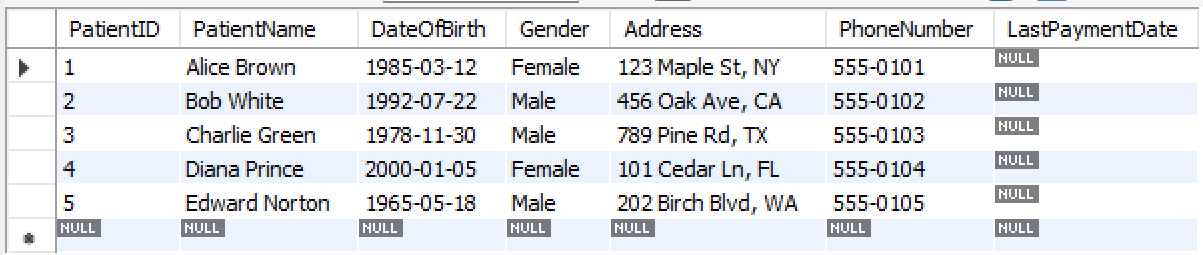
\includegraphics[width=0.8\textwidth]{Images/sample_patients.png}
    \caption{\texttt{Patients} sample data}
    \label{fig:sample_patients}
\end{figure}

\subsubsection*{Doctors}
\begin{figure}[H]
    \centering
    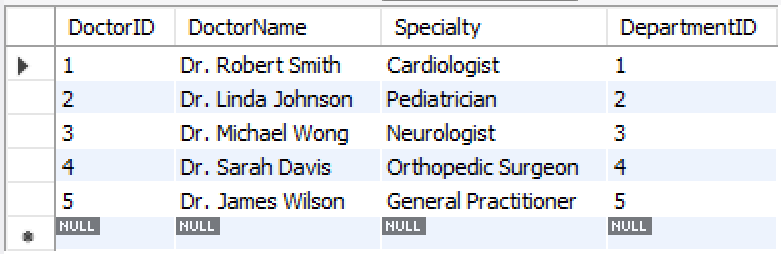
\includegraphics[width=0.7\textwidth]{Images/sample_doctors.png}
    \caption{\texttt{Doctors} sample data}
    \label{fig:sample_doctors}
\end{figure}

\subsubsection*{Departments}
\begin{figure}[H]
    \centering
    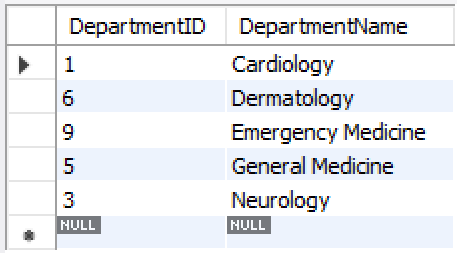
\includegraphics[width=0.5\textwidth]{Images/sample_departments.png}
    \caption{\texttt{Departments} sample data}
    \label{fig:sample_departments}
\end{figure}

\subsubsection*{Appointments}
\begin{figure}[H]
    \centering
    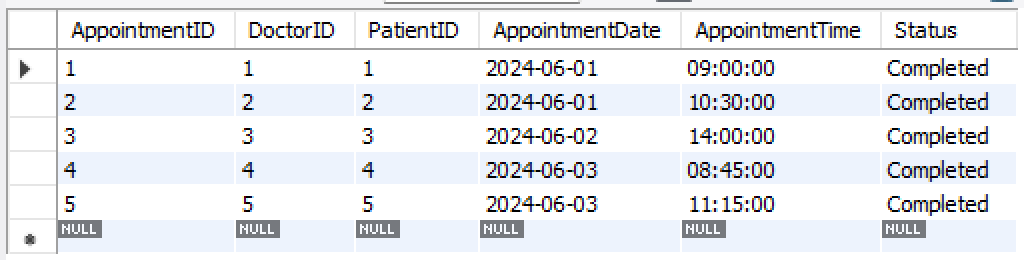
\includegraphics[width=0.8\textwidth]{Images/sample_appointments.png}
    \caption{\texttt{Appointments} sample data}
    \label{fig:sample_appointments}
\end{figure}

\subsubsection*{Invoices}
\begin{figure}[H]
    \centering
    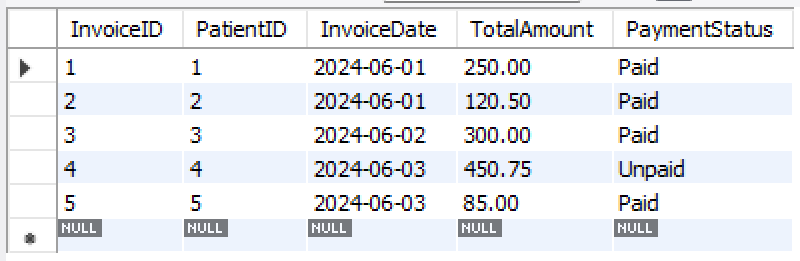
\includegraphics[width=0.7\textwidth]{Images/sample_invoices.png}
    \caption{\texttt{Invoices} sample data}
    \label{fig:sample_invoices}
\end{figure}

\subsubsection*{AuditLog}
\begin{figure}[H]
    \centering
    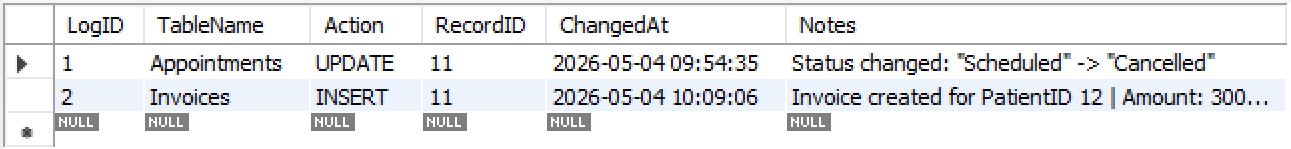
\includegraphics[width=0.9\textwidth]{Images/sample_auditlog.png}
    \caption{\texttt{AuditLog} sample data}
    \label{fig:sample_auditlog}
\end{figure}

\subsection{Database Diagram}

This section presents the visual blueprint of the physical database as implemented in the MySQL environment. The Enhanced Entity-Relationship (EER) diagram was generated directly from MySQL Workbench to provide a precise representation of the final schema.

\begin{figure}[h!]
    \centering
    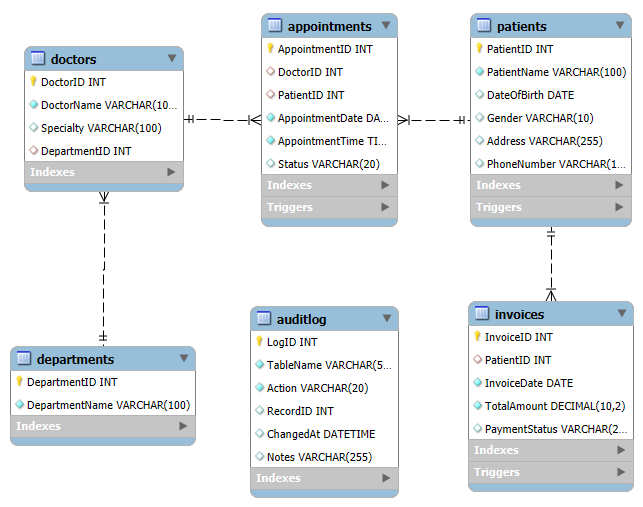
\includegraphics[width=0.8\textwidth]{Images/eer.png}
    \caption{Enhanced Entity-Relationship (EER) Diagram from MySQL Workbench}
    \label{fig:eer_diagram}
\end{figure}

The diagram serves as a technical reference for the system's architecture, highlighting the following key elements:
\begin{itemize}
    \item \textbf{Table Structures:} Displays specific data types like INT and VARCHAR for all columns.
    \item \textbf{Physical Constraints:} Defines Primary Keys and Foreign Keys to ensure data integrity across the schema.
    \item \textbf{Relationship Mapping:} Illustrates one to many cardinality and referential paths for core operational entities.
     \item \textbf{System Auditing:} Includes a standalone AuditLog table to record historical data modifications.
\end{itemize}